\documentclass{article}
\usepackage{ucs}
\usepackage[utf8x]{inputenc}
\usepackage[T1]{fontenc}
\usepackage[ngerman]{babel}
\usepackage{pdfpages}
\usepackage{graphicx}
\usepackage{hyperref}
\usepackage{cite}
\usepackage{pdfpages}
\usepackage{rotating}

\title{
Frage zur Berechnung der Gradienten, LH-Werte.
}

%\date{14.06.2018}
\author{Lukas Diewald, lukas.diewald@student.kit.edu}


\begin{document}

Frage 1 :
\newline
Im Paper von Hong \cite{hong2003method} wird für jeden Voxel der Gradient mithilfe seiner 64 Nachbarkanten bestimmt(siehe Abbildung).
In meinem Fall sind jedoch die Intensitätswerte in den Voxelzentren und nicht in den Kanten gespeichert.
Meine Frage wäre, ist es sinnvoller das Volumenmodel umzurechnen, dass die Werte in den Kanten gespeichert werden.
Beispielsweise indem man den Wert einer Kante aus den 8 umliegenden Voxel berechnet.
Oder sollte ich lieber statt den 64 Nachbarkanten die 26 Nachbarvoxel in die Berechnung einbeziehen?

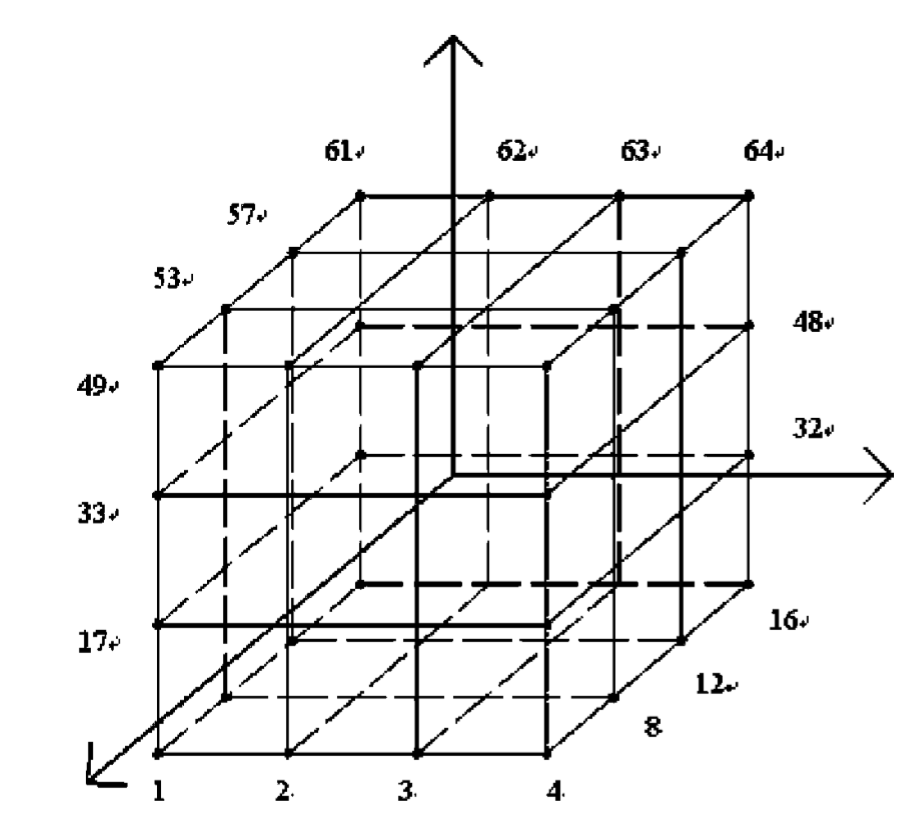
\includegraphics[width=0.7\textwidth]{VoxelEdges.PNG}
.
\newline
Frage 2:
\newline
In der Arbeit von Binh P. Nguyen \cite{nguyen2011automatic} werden mithilfe von den Gradienten die LH-Werte jedes Voxels berechnet. Hierbei wird in beide Richtungen integriert unter der Verwendung von Heun's Verfahren. Es wird folgende Formel verwendet:
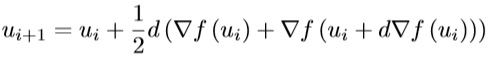
\includegraphics[width=0.8\textwidth]{Formula.PNG}

Wobei Ui und Ui+1 der aktuell betrachtete und der nächste Voxel, f der normalisierte Gradient des jeweiligen Voxels und d die Schrittweiten, in diesem Fall ein Voxel, ist.
Die Integration stoppt, wenn ein lokaes Extremum oder ein Wendepunkt gefunden wird.
Meine Frage dazu ist, wie erkenne ich ein solchen Punkt mithilfe der Gradienten und dem berechneten Pfad?

\bibliography{Frage}{}
\bibliographystyle{plain}



\end{document}